\documentclass[journal,12pt,twocolumn]{IEEEtran}
%
\usepackage{setspace}
\usepackage{gensymb}
\usepackage{siunitx}
\usepackage{tkz-euclide} 
\usepackage{textcomp}
\usepackage{standalone}
\usetikzlibrary{calc}
\newcommand\hmmax{0}
\newcommand\bmmax{0}

%\doublespacing
\singlespacing

%\usepackage{graphicx}
%\usepackage{amssymb}
%\usepackage{relsize}
\usepackage[cmex10]{amsmath}
%\usepackage{amsthm}
%\interdisplaylinepenalty=2500
%\savesymbol{iint}
%\usepackage{txfonts}
%\restoresymbol{TXF}{iint}
%\usepackage{wasysym}
\usepackage{amsthm}
%\usepackage{iithtlc}
\usepackage{mathrsfs}
\usepackage{txfonts}
\usepackage{stfloats}
\usepackage{bm}
\usepackage{cite}
\usepackage{cases}
\usepackage{subfig}
%\usepackage{xtab}
\usepackage{longtable}
\usepackage{multirow}
%\usepackage{algorithm}
%\usepackage{algpseudocode}
\usepackage{enumitem}
\usepackage{mathtools}
\usepackage{steinmetz}
\usepackage{tikz}
\usepackage{circuitikz}
\usepackage{verbatim}
\usepackage{tfrupee}
\usepackage[breaklinks=true]{hyperref}
%\usepackage{stmaryrd}
\usepackage{tkz-euclide} % loads  TikZ and tkz-base
%\usetkzobj{all}
\usetikzlibrary{calc,math}
\usepackage{listings}
    \usepackage{color}                                            %%
    \usepackage{array}                                            %%
    \usepackage{longtable}                                        %%
    \usepackage{calc}                                             %%
    \usepackage{multirow}                                         %%
    \usepackage{hhline}                                           %%
    \usepackage{ifthen}                                           %%
  %optionally (for landscape tables embedded in another document): %%
    \usepackage{lscape}     
\usepackage{multicol}
\usepackage{chngcntr}
\usepackage{amsmath}
\usepackage{cleveref}
\usepackage{amsmath}
%\usepackage{enumerate}

%\usepackage{wasysym}
%\newcounter{MYtempeqncnt}
\DeclareMathOperator*{\Res}{Res}
%\renewcommand{\baselinestretch}{2}
\renewcommand\thesection{\arabic{section}}
\renewcommand\thesubsection{\thesection.\arabic{subsection}}
\renewcommand\thesubsubsection{\thesubsection.\arabic{subsubsection}}

\renewcommand\thesectiondis{\arabic{section}}
\renewcommand\thesubsectiondis{\thesectiondis.\arabic{subsection}}
\renewcommand\thesubsubsectiondis{\thesubsectiondis.\arabic{subsubsection}}

% correct bad hyphenation here
\hyphenation{op-tical net-works semi-conduc-tor}
\def\inputGnumericTable{}                                 %%

\lstset{
%language=C,
frame=single, 
breaklines=true,
columns=fullflexible
}
%\lstset{
%language=tex,
%frame=single, 
%breaklines=true
%}
\usepackage{graphicx}
\usepackage{pgfplots}

\begin{document}


\newtheorem{theorem}{Theorem}[section]
\newtheorem{problem}{Problem}
\newtheorem{proposition}{Proposition}[section]
\newtheorem{lemma}{Lemma}[section]
\newtheorem{corollary}[theorem]{Corollary}
\newtheorem{example}{Example}[section]
\newtheorem{definition}[problem]{Definition}
%\newtheorem{thm}{Theorem}[section] 
%\newtheorem{defn}[thm]{Definition}
%\newtheorem{algorithm}{Algorithm}[section]
%\newtheorem{cor}{Corollary}
\newcommand{\BEQA}{\begin{eqnarray}}
\newcommand{\EEQA}{\end{eqnarray}}
\newcommand{\define}{\stackrel{\triangle}{=}}
\bibliographystyle{IEEEtran}
%\bibliographystyle{ieeetr}
\providecommand{\mbf}{\mathbf}
\providecommand{\abs}[1]{\ensuremath{\left\vert#1\right\vert}}
\providecommand{\norm}[1]{\ensuremath{\left\lVert#1\right\rVert}}
\providecommand{\mean}[1]{\ensuremath{E\left[ #1 \right]}}
\providecommand{\pr}[1]{\ensuremath{\Pr\left(#1\right)}}
\providecommand{\qfunc}[1]{\ensuremath{Q\left(#1\right)}}
\providecommand{\sbrak}[1]{\ensuremath{{}\left[#1\right]}}
\providecommand{\lsbrak}[1]{\ensuremath{{}\left[#1\right.}}
\providecommand{\rsbrak}[1]{\ensuremath{{}\left.#1\right]}}
\providecommand{\brak}[1]{\ensuremath{\left(#1\right)}}
\providecommand{\lbrak}[1]{\ensuremath{\left(#1\right.}}
\providecommand{\rbrak}[1]{\ensuremath{\left.#1\right)}}
\providecommand{\cbrak}[1]{\ensuremath{\left\{#1\right\}}}
\providecommand{\lcbrak}[1]{\ensuremath{\left\{#1\right.}}
\providecommand{\rcbrak}[1]{\ensuremath{\left.#1\right\}}}
\theoremstyle{remark}
\newtheorem{rem}{Remark}
\newcommand{\sgn}{\mathop{\mathrm{sgn}}}
\providecommand{\res}[1]{\Res\displaylimits_{#1}} 
%\providecommand{\norm}[1]{\lVert#1\rVert}
\providecommand{\mtx}[1]{\mathbf{#1}}
\providecommand{\fourier}{\overset{\mathcal{F}}{ \rightleftharpoons}}
%\providecommand{\hilbert}{\overset{\mathcal{H}}{ \rightleftharpoons}}
\providecommand{\system}{\overset{\mathcal{H}}{ \longleftrightarrow}}
	%\newcommand{\solution}[2]{\textbf{Solution:}{#1}}
\newcommand{\solution}{\noindent \textbf{Solution: }}
\newcommand{\cosec}{\,\text{cosec}\,}
\providecommand{\dec}[2]{\ensuremath{\overset{#1}{\underset{#2}{\gtrless}}}}
\newcommand{\myvec}[1]{\ensuremath{\begin{pmatrix}#1\end{pmatrix}}}
\newcommand{\mydet}[1]{\ensuremath{\begin{vmatrix}#1\end{vmatrix}}}
%\numberwithin{equation}{section}
\numberwithin{equation}{subsection}
%\numberwithin{problem}{section}
%\numberwithin{definition}{section}
\makeatletter
\@addtoreset{figure}{problem}
\makeatother
\let\StandardTheFigure\thefigure
\let\vec\mathbf
%\renewcommand{\thefigure}{\theproblem.\arabic{figure}}
\renewcommand{\thefigure}{\theproblem}
%\setlist[enumerate,1]{before=\renewcommand\theequation{\theenumi.\arabic{equation}}
%\counterwithin{equation}{enumi}
%\renewcommand{\theequation}{\arabic{subsection}.\arabic{equation}}
\def\putbox#1#2#3{\makebox[0in][l]{\makebox[#1][l]{}\raisebox{\baselineskip}[0in][0in]{\raisebox{#2}[0in][0in]{#3}}}}
     \def\rightbox#1{\makebox[0in][r]{#1}}
     \def\centbox#1{\makebox[0in]{#1}}
     \def\topbox#1{\raisebox{-\baselineskip}[0in][0in]{#1}}
\vspace{3cm}
\title{Polynomial Curve Fitting}
\maketitle
\newpage
%\tableofcontents
\bigskip
\renewcommand{\thefigure}{\theenumi}
\renewcommand{\thetable}{\theenumi}
\begin{abstract}
This document contains theory involved in curve fitting.
\end{abstract}
\section{\textbf{Objective}}
The objective is to fit best line for the polynomial curve using regularization.
\section{Generate Dataset}
Create a sinusoidal function of the form
\begin{align}
    y = A\sin{2\pi x} + n(t) \label{eq:1}
\end{align}
n(t) is the random noise that is included in the training set. This set consists of N samples of input data i.e. x expressed as shown below
\begin{align}
    x = \myvec{x_{1}, x_{2}, .., x_{N}}^{T}
\end{align}
which give the corresponding values of y denoted as
\begin{align}
    y = \myvec{y_{1}, y_{2}, .., y_{N}}^{T}
\end{align}
\begin{figure}[!h]
\begin{center}
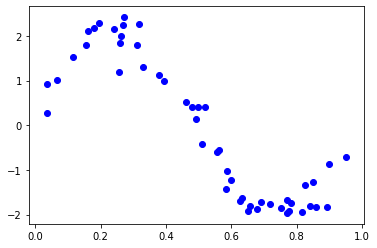
\includegraphics[width=3.4in]{figs/fig1.png}
\end{center}
\caption{Sinusoidal Dataset with added noise}
\label{fig:1}
\end{figure}
The Fig \ref{fig:1} is generated by random values of $x_{n}$ for n =1,2,..,N.
where N=50 in the range [0,1].

The corresponding values of y were generated from the Eq \eqref{eq:1}.The first term $A\sin{2\pi x}$ is computed directly and then random noise samples having a normal(Gaussian) distribution are added inorder to get the corresponding values of y.
\begin{lstlisting}
#Generate the sine curve 
import numpy as np
import matplotlib.pyplot as plt

N = 50
np.random.seed(20)
x = np.sort(np.random.rand(N,1),axis=0)
noise = np.random.normal(0,0.3,size=(N,1))
A = 2.5
y = A*np.sin(2*np.pi*x) + noise

plt.scatter(x,y,c='b',marker='o',label='Data with noise')
plt.xlabel('x');plt.ylabel('y')
\end{lstlisting}

The following code generates the input matrix F
\begin{lstlisting}
sk_poly_deg=3
poly_feature = PolynomialFeatures(degree=sk_poly_deg,include_bias=False)
F = poly_feature.fit_transform(x)
\end{lstlisting}

The generated matrix would look like
\begin{align}
    \vec{F}= \myvec{ 1 & x_{0} & x_{0}^2 & \ldots & x_{0}^{N-1} \\
		1 & x_{1} & x_{1}^2 & \ldots & x_{1}^{N-1} \\
		1 & x_{2} & x_{2}^2 & \ldots & x_{2}^{N-1} \\
		\vdots & & \vdots &  & \vdots  \\
		    1 & \ldots & \ldots & \ldots & x_{N}^{N-1} }\label{eq:12}
\end{align}
\section{Polynomial Curve Fitting}
The goal is to find the best line that fits into the  pattern of the training data shown in the graph.
We shall fit the data using a polynomial function of the form, 
\begin{align}
     y\brak{w,x}= \sum_{j=0}^{M} w_j x^{j}\\
\end{align}
M is the order of the polynomial
The polynomial coefficient are collectively denoted by the vector $\vec{w}$.The proposed vector $\vec{w}$ of the model referring to Eq \eqref{eq:12} is given by 
\begin{align}
    \hat{\vec{w}} = \brak{\vec{F}^T\vec{F}}^{-1}\vec{F}^Ty \label{eq:13}
\end{align}

\section{Bias- Variance Tradeoff}
In decision theory, the decision stage consists of choosing a specific estimate $y(\vec{x})$ for the target t for each input $\vec{x}$

This can be done by using a loss function $L(t,y(\vec{x}))$ so the expected loss is
\begin{align}
    E[L] = \int \int L(t,y(\vec{x}))p(\vec{x},t)d\vec{x}dt
\end{align}
A common loss function is the squared loss function given by
\begin{align}
    L(t,y(\vec{x})) = (y(\vec{x}) - t)^2 \label{eq : squared_loss_func}
\end{align}
The expected loss for Eq \eqref{eq : squared_loss_func},
\begin{align}
    E[L] = \int \int (y(\vec{x}) - t)^2p(\vec{x},t)d\vec{x}dt
\end{align}
The optimal prediction for the squared loss function is given by the conditional expectation h(x)
\begin{align}
    h(x) = E[t |\vec{x}] = \int t p(t |\vec{x})dt
\end{align}
where $p(t | \vec{x})$ is the conditional distribution

The expected square loss takes the form
\begin{multline}
    E[L] = \int(y(\vec{x})-h(\vec{x}))^2p(\vec{x})d\vec{x} +\\ 
    \int \int(h(\vec{x}) - t)^2p(\vec{x},t)d\vec{x} dt \label{eq : expected_loss}
\end{multline}
In Eq \eqref{eq : expected_loss},
Second term is due to the noise in the data.

Consider the integrand of the first term in Eq \eqref{eq : expected_loss}, which becomes
\begin{align}
    (y(\vec{x};D) - h(\vec{x}))^2 \label{eq : first_term}
\end{align}
for D data sets.

Adding and subtracting $E[y(\vec{x};D)]$ to Eq \eqref{eq : first_term}
\begin{align}
    (y(\vec{x};D) - E[y(\vec{x};D)] + E[y(\vec{x};D)]- h(\vec{x}))^2
\end{align}
Expanding,
\begin{multline}
    \brak{y(\vec{x};D) - E[y(\vec{x};D)] + E[y(\vec{x};D)]- h(\vec{x})}^2 = \\
      \brak{y(\vec{x};D) - E[y(\vec{x};D)]}^2 + \brak{E[y(\vec{x};D)]- h(\vec{x})}^2 + \\
      2\brak{y(\vec{x};D) - E[y(\vec{x};D)]}\brak{E[y(\vec{x};D)]- h(\vec{x})}^2)
\end{multline}
Take the expectation w.r.t D,
\begin{multline}
    E[(y(\vec{x};D) - h(\vec{x}))^2] = \brak{E[y(\vec{x};D)]- h(\vec{x})}^2\\
       + E_{D}[(y(\vec{x};D) - E_{D}[y(\vec{x};D)])^2] \label{eq : modified_expected}
\end{multline}
In Eq \eqref{eq : modified_expected}, 

First term -  $(bias)^2$ 

Second term - $variance$ 

Now substituting this expanded eq in Eq \eqref{eq : expected_loss},
$expected loss = (bias)^2 + variance + noise$

\begin{align}
    (bias)^2 = \int \brak{E[y(\vec{x};D)]- h(\vec{x})}^2 p(\vec{x}) d\vec{x}\\
    variance = \int E_{D}[(y(\vec{x};D) - E_{D}[y(\vec{x};D)])^2] p(\vec{x}) d\vec{x}\\
    noise = \int(h(\vec{x}) - t)^2p(\vec{x},t)d\vec{x} dt
\end{align}
The ultimate goal is to minimize the expected loss which we have decomposed into $(bias)^2$, $variance$ and constant noise term.

\section{Example}
We generate 100 datasets, each containing 50 data points independently from the sinusoidal curve $h(x) = sin(2\pi x)$ . 

For each dataset, we fit the model by using regularization.

large $\lambda$, low variance but high bias and

small $\lambda$, low bias but high variance.

We have to choose to $\lambda$ value such that the value of $(bias)^2 + variance$ is minimum.

Plots for different values of $\lambda$.

\begin{figure}[!h]
\begin{center}
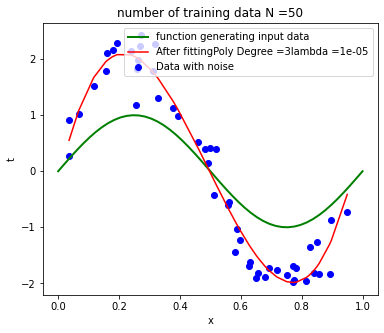
\includegraphics[width=3.4in]{figs/fig2.png}
\end{center}
\caption{}
\label{fig:2}
\end{figure}

\begin{figure}[!h]
\begin{center}
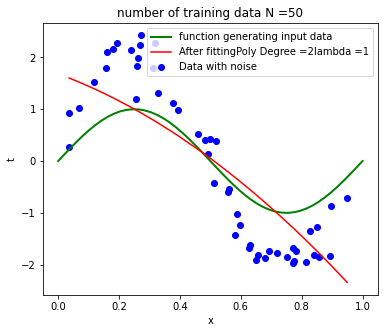
\includegraphics[width=3.4in]{figs/fig3.png}
\end{center}
\caption{}
\label{fig:3}
\end{figure}

\begin{figure}[!h]
\begin{center}
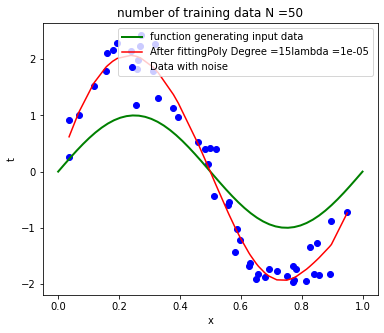
\includegraphics[width=3.4in]{figs/fig4.png}
\end{center}
\caption{}
\label{fig:4}
\end{figure}

\begin{figure}[!h]
\begin{center}
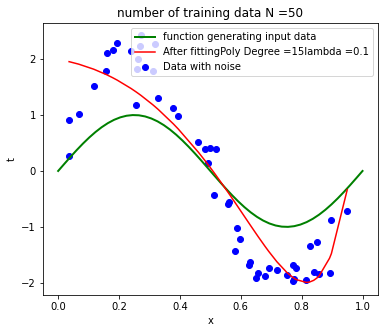
\includegraphics[width=3.4in]{figs/fig5.png}
\end{center}
\caption{}
\label{fig:5}
\end{figure}

The average prediction is estimated from
\begin{align}
    \bar y(\vec{x}) = \frac{1}{L} \sum_{l=1}^{L} y^{(l)}(\vec{x})
\end{align}
and the integrated $(bias)^2$ and variance is given by
\begin{align}
    (bias)^2 = \frac{1}{N} \sum_{n=1}^{N} \brak{\bar y(x_{n}) - h(x_{n})}^2\\
    variance = \frac{1}{N} \sum_{n=1}^{N} \frac{1}{L} \sum_{l=1}^{L} \brak{y^{(l)}(x_{n}) - \bar y(x_{n})}
\end{align}
The model with optimal predictive capability is the one with best balance.

Python code:
\begin{lstlisting}
https://github.com/Hrithikraj2/EE4015_IDP/blob/main/Assignment_5/Assignment_5.ipynb
\end{lstlisting}
\end{document}
